
% ------------------------ Prototype ------------------------

\section*{APPENDIX A - Prototype \label{sec:proto}}
\addcontentsline{toc}{section}{APPENDIX A - Prototype}


\begin{comment}

    Provide the filtered part of RM showing selected features for prototype building. State the detailed steps of compilation, execution and setups. Specify prototype details showing codes, screens, test data, sample output and detailed steps of compilation, execution and setups (if any).

\end{comment}

% ---------- Start the prototype appendix
\noindent
Below is a Sequence Diagram of the Application. The diagram shows the flow of the application when a user interacts with it. The user can either enter text, upload an image, upload a video, or analyze a Reddit or Twitter user. The application then processes the input and provides the user with the result. The user can also retrain the model using the Reddit data. The application also provides the user with the option to analyze facial expressions and generate image captions. The application also generates a knowledge graph based on the classification result.

\begin{figure}[h!]  
    \centering
    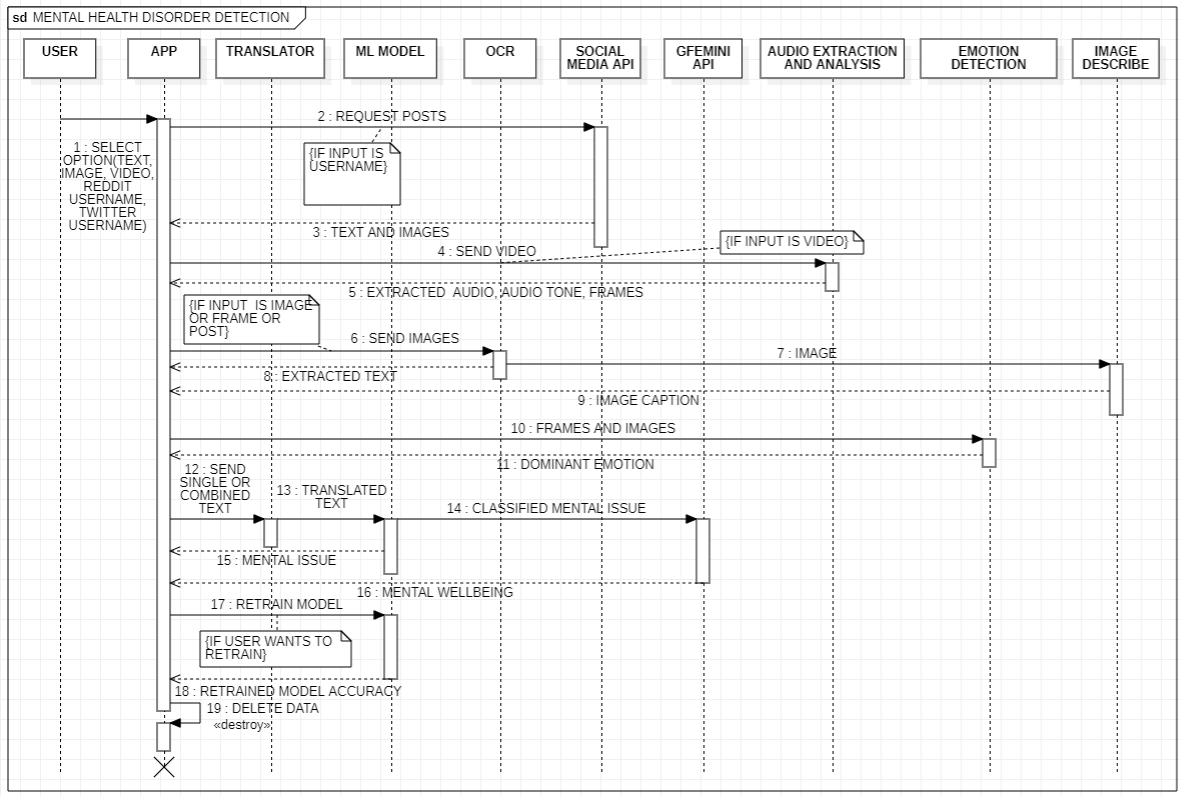
\includegraphics[width=1.0\textwidth]{Images/Sequence Diagram.png}  
    \caption{Sequence Diagram of the Application}
    \label{012i}  % Label for referencing the figure
\end{figure}

\noindent
Lets see the working of each of the five options of the application when an input is given through diagrams below. The first option is to enter text for classification. The user enters the text and the application classifies the text into one of the categories. The second option is to upload an image. The user uploads an image and the application classifies the image into one of the categories. The third option is to upload a video. The user uploads a video and the application classifies the video into one of the categories. The fourth option is to analyze a Reddit user. The user enters the Reddit username and the application analyzes the Reddit user. The fifth option is to analyze a Twitter user. The user enters the Twitter username and the application analyzes the Twitter user.

\pagebreak

\begin{figure}[h!]  
    \centering
    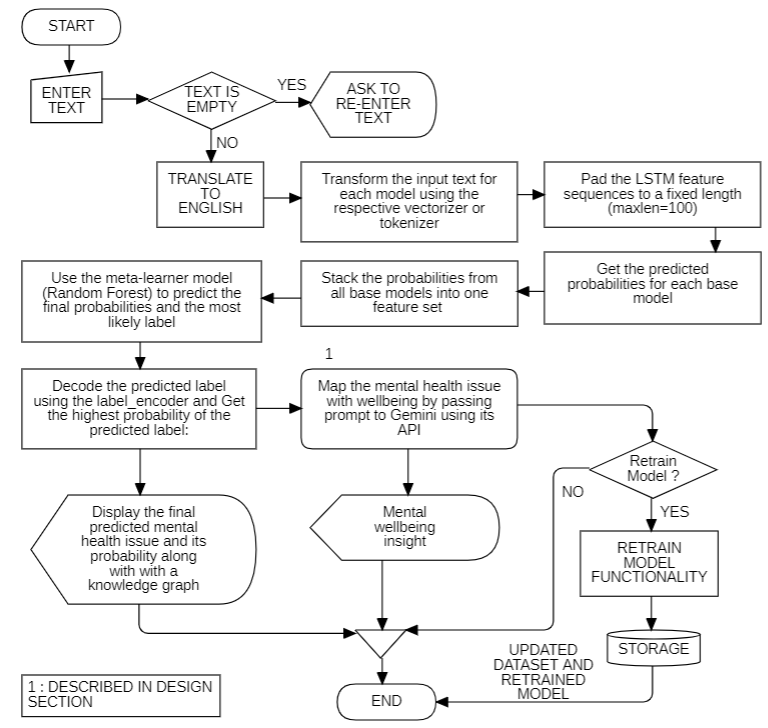
\includegraphics[width=1.0\textwidth]{Images/APP TEXT OPTION.png}  
    \caption{Text Classification Flow Diagram}
    \label{012i}  % Label for referencing the figure
\end{figure}


\pagebreak
\begin{figure}[h!]  
    \centering
    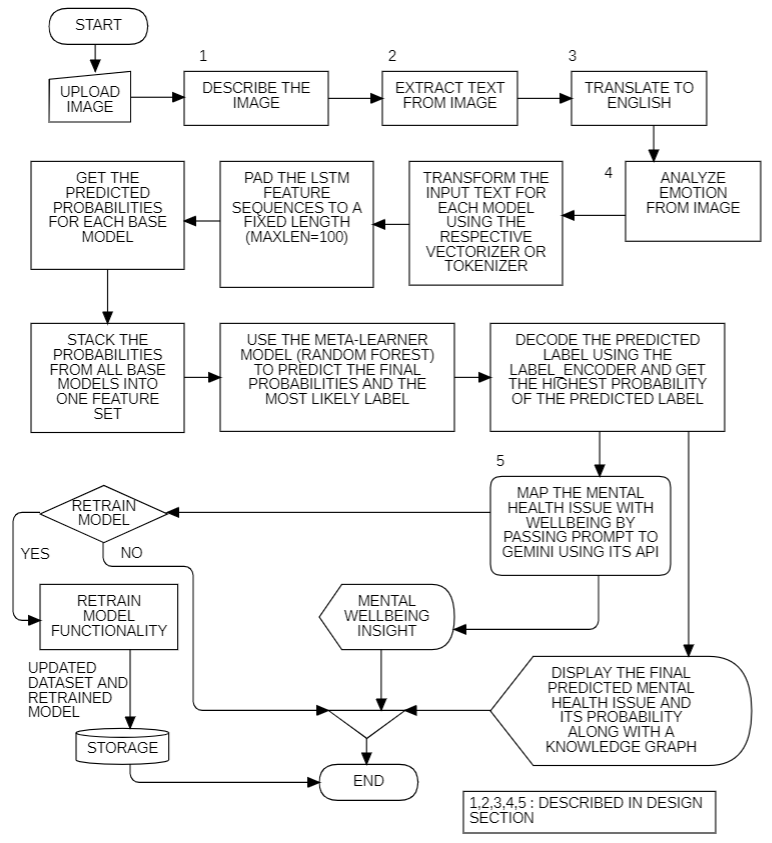
\includegraphics[width=1.0\textwidth]{Images/APP IMAGE OPTION.png}  
    \caption{Image Classification Flow Diagram}
    \label{011232i}  % Label for referencing the figure
\end{figure}

\pagebreak
\begin{figure}[h!]  
    \centering
    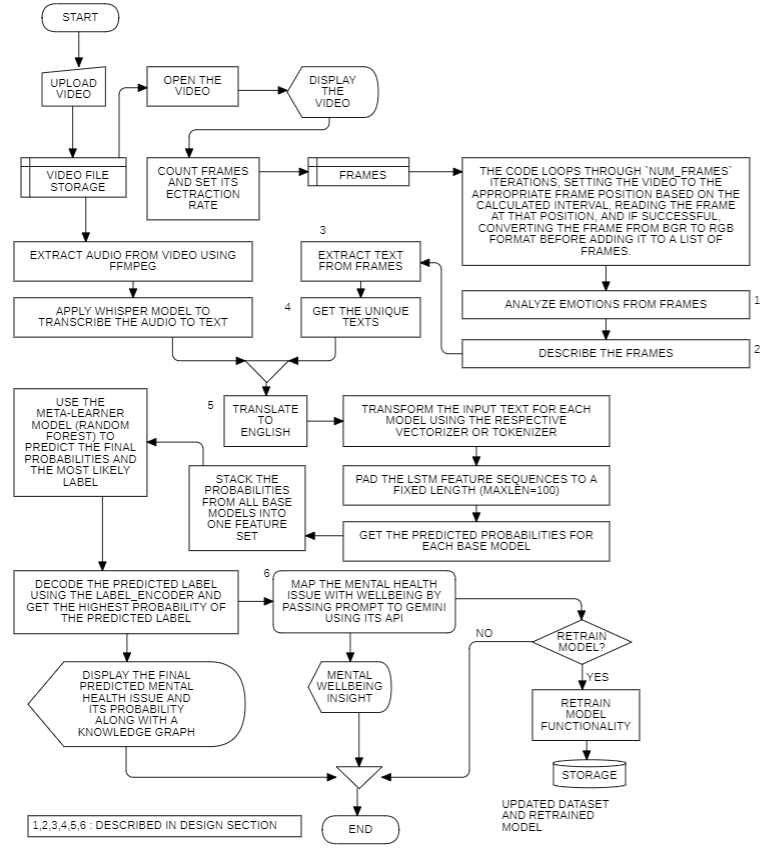
\includegraphics[width=1.0\textwidth]{Images/APP VIDEO OPTION.png}  
    \caption{Video Classification Flow Diagram}
    \label{01332i}  % Label for referencing the figure
\end{figure}

\pagebreak
\begin{figure}[h!]  
    \centering
    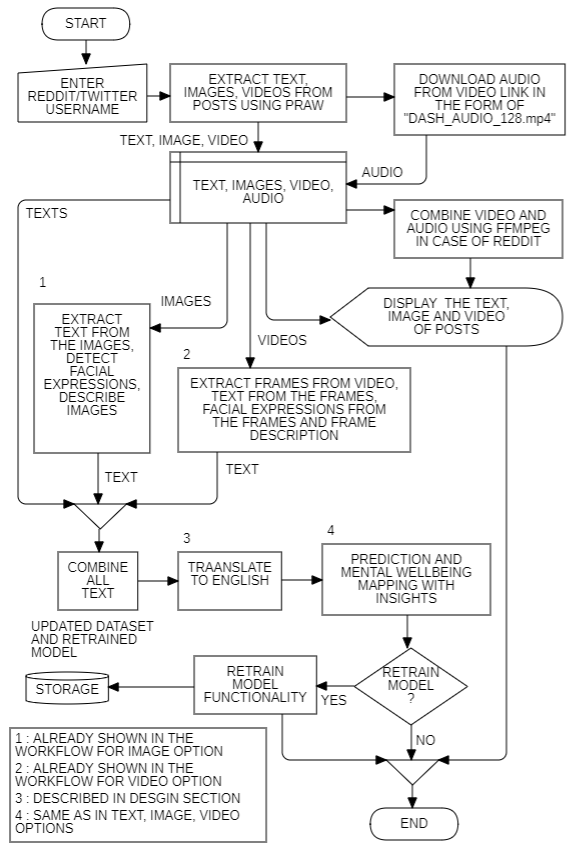
\includegraphics[width=0.9\textwidth]{Images/APP REDDIT.png}  
    \caption{Reddit and Twitter username Classification Flow Diagram}
    \label{01234i}  % Label for referencing the figure
\end{figure}

\pagebreak
\noindent
Below are some screenshots from the web application.

\begin{figure}[h!]  
    \centering
    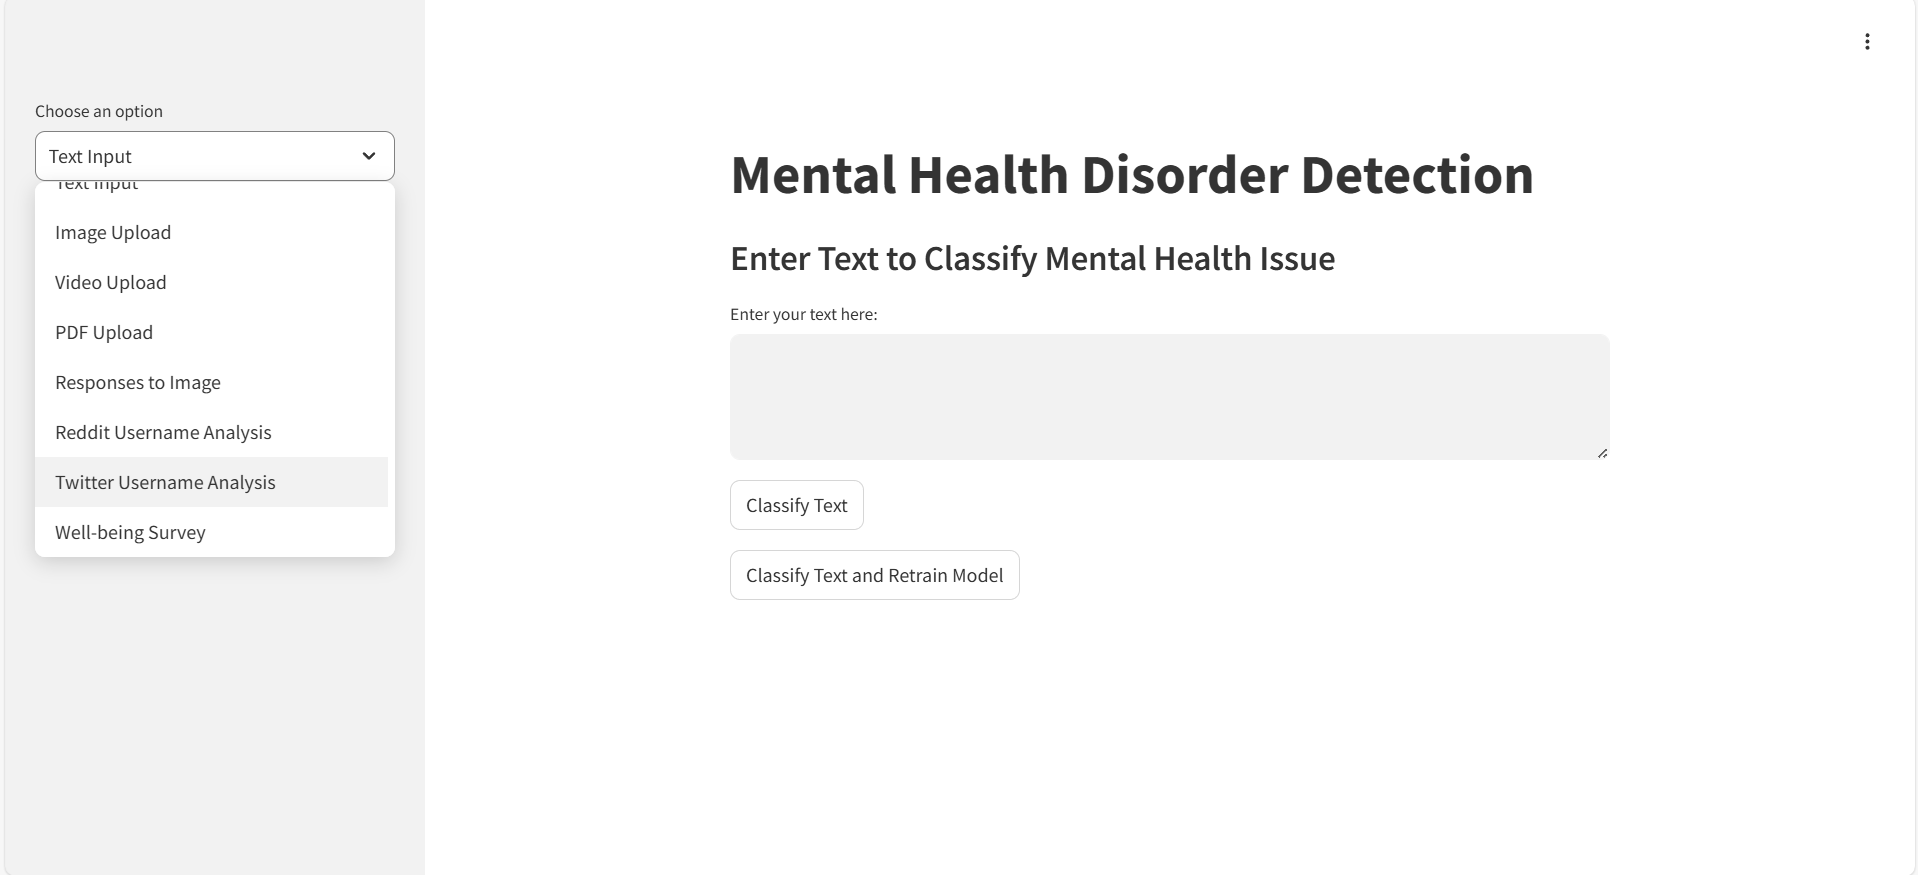
\includegraphics[width=0.8\textwidth]{App Images/01 Interface.png}  
    \caption{Website with all options}
    \label{01i}  % Label for referencing the figure
\end{figure}

\begin{figure}[h!]  
    \centering
    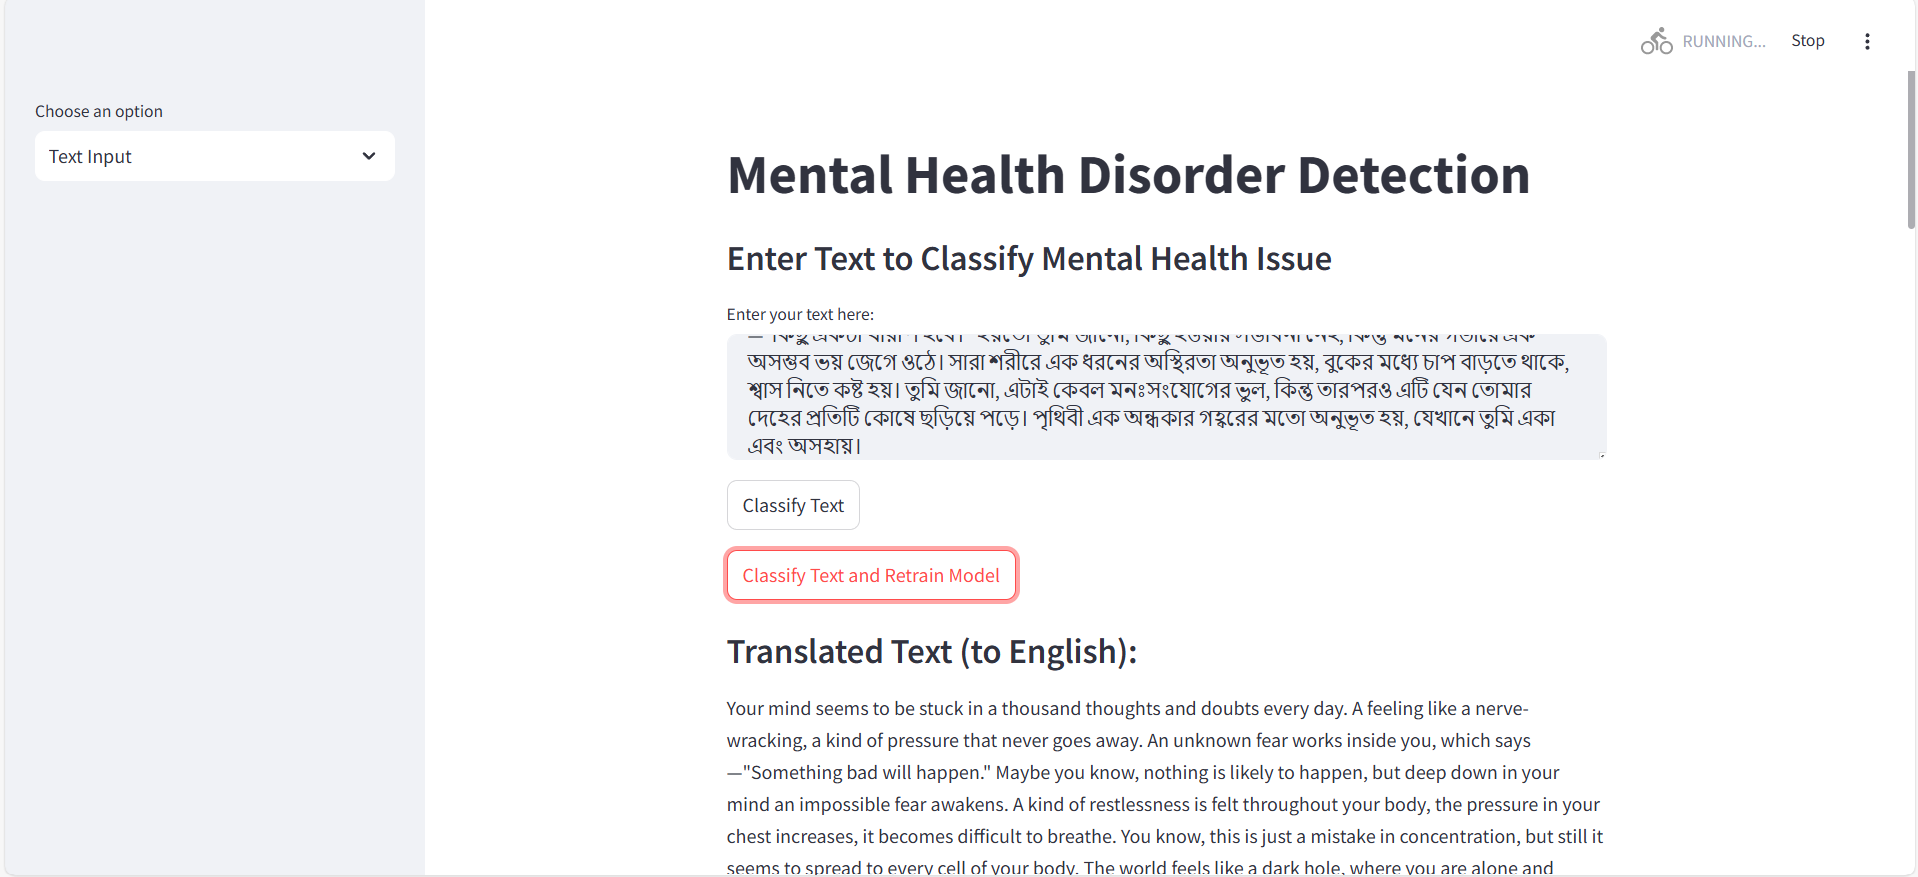
\includegraphics[width=0.8\textwidth]{App Images/02 Interface.png}  
    \caption{Entering Text for classification}
    \label{02i}  % Label for referencing the figure
\end{figure}

\begin{figure}[h!]  
    \centering
    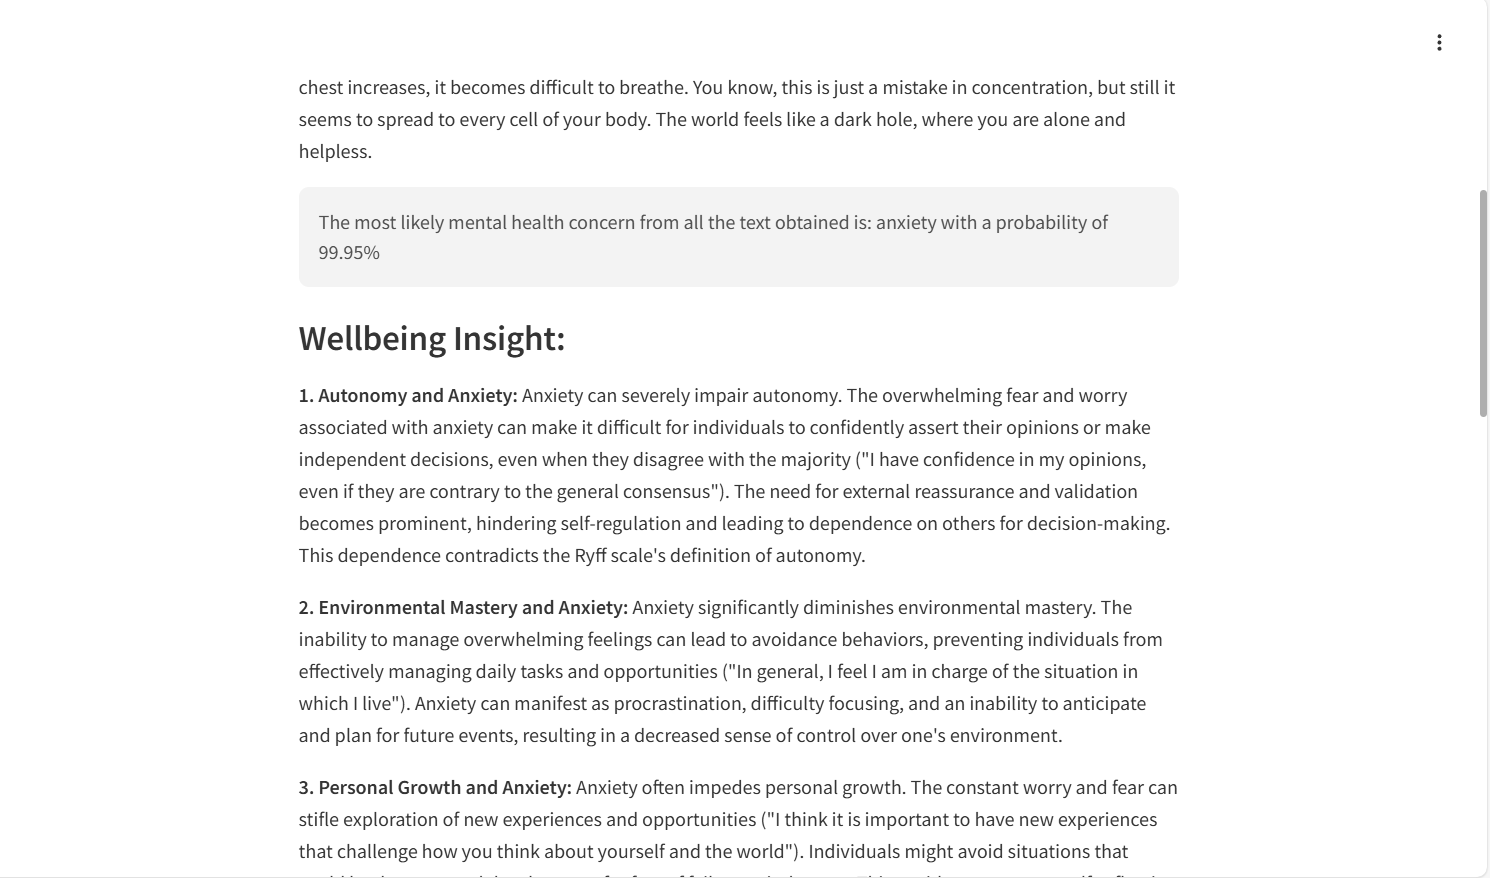
\includegraphics[width=0.8\textwidth]{App Images/03 Interface.png}  
    \caption{Text Classification Result}
    \label{03i}  % Label for referencing the figure
\end{figure}



\begin{figure}[h!]  
    \centering
    
\includegraphics[width=0.8\textwidth]{App Images/04 Interface.png}  
    \caption{Upload Image}
    \label{04i}  % Label for referencing the figure
\end{figure}

\begin{figure}[h!]  
    \centering
    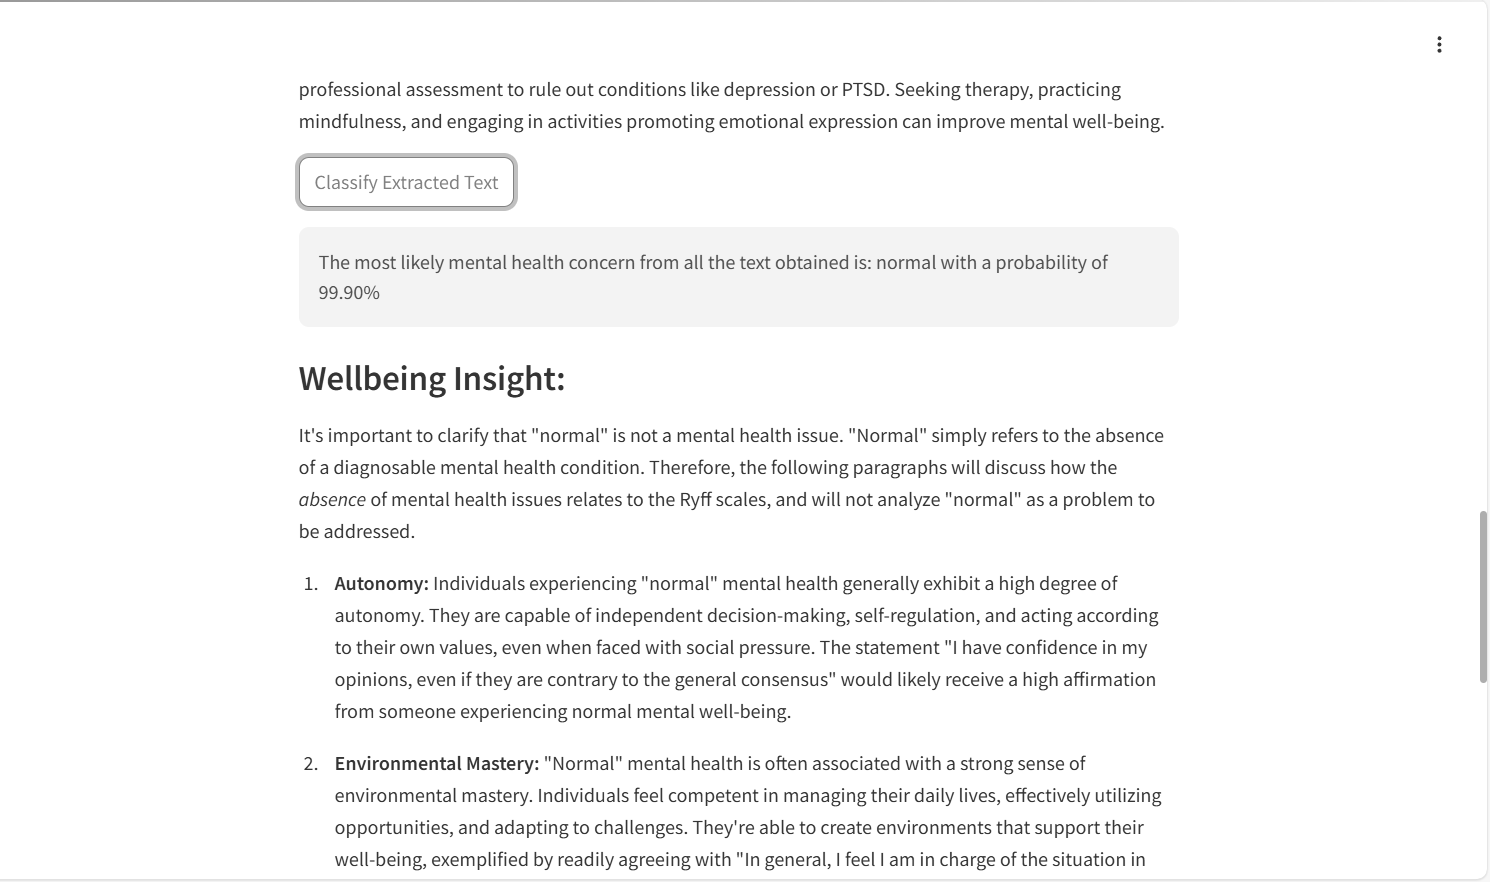
\includegraphics[width=0.8\textwidth]{App Images/05 Interface.png}  
    \caption{Image Classification Result}
    \label{05i}  % Label for referencing the figure
\end{figure}


\begin{figure}[h!]  
    \centering
    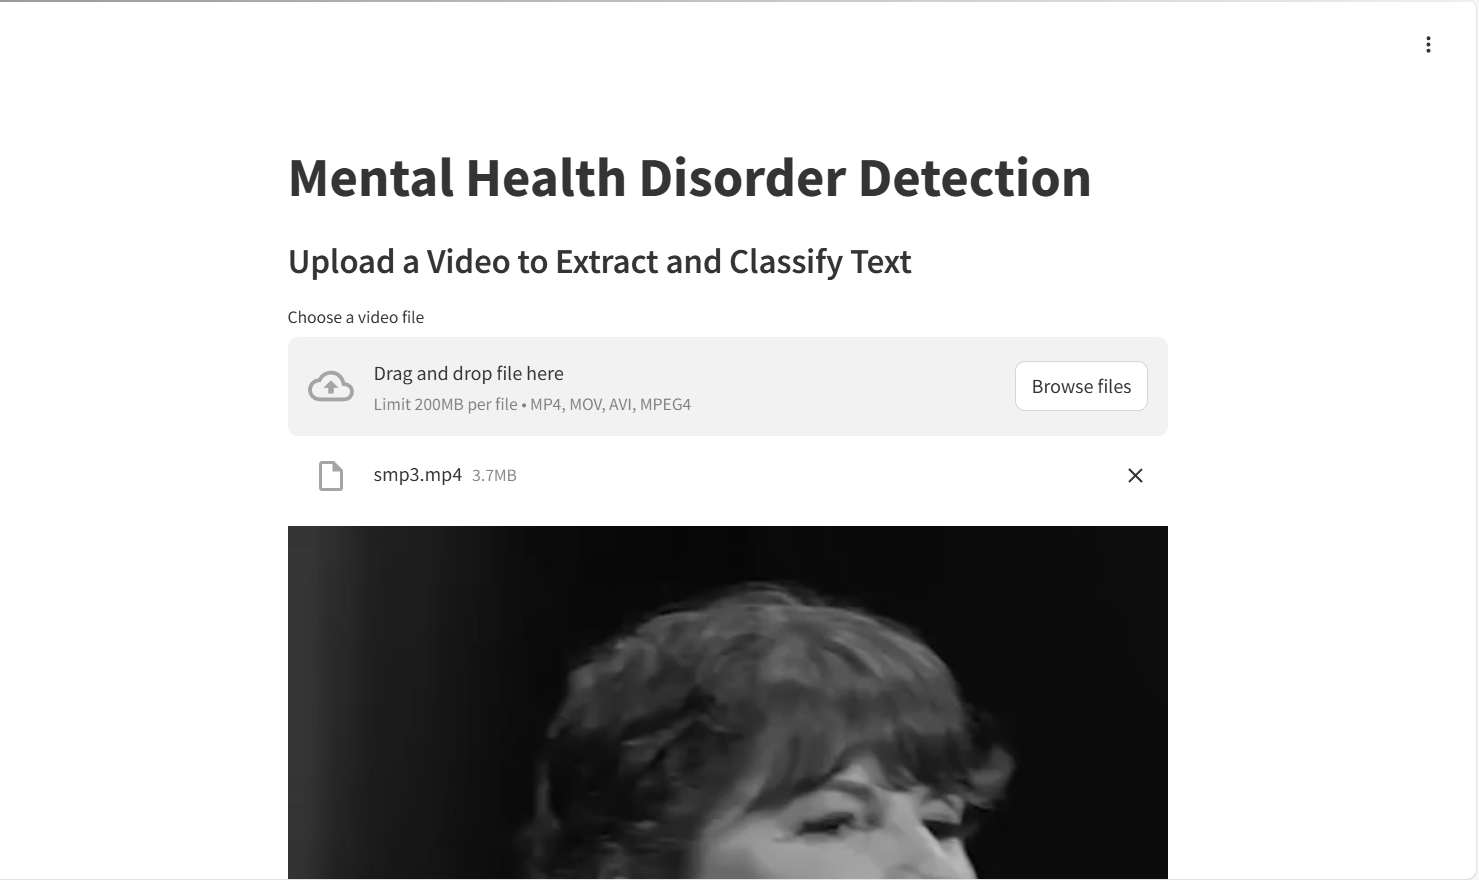
\includegraphics[width=0.8\textwidth]{App Images/12 Interface.png}  
    \caption{Upload Video}
    \label{06i4}  % Label for referencing the figure
\end{figure}

\begin{figure}[h!]  
    \centering
    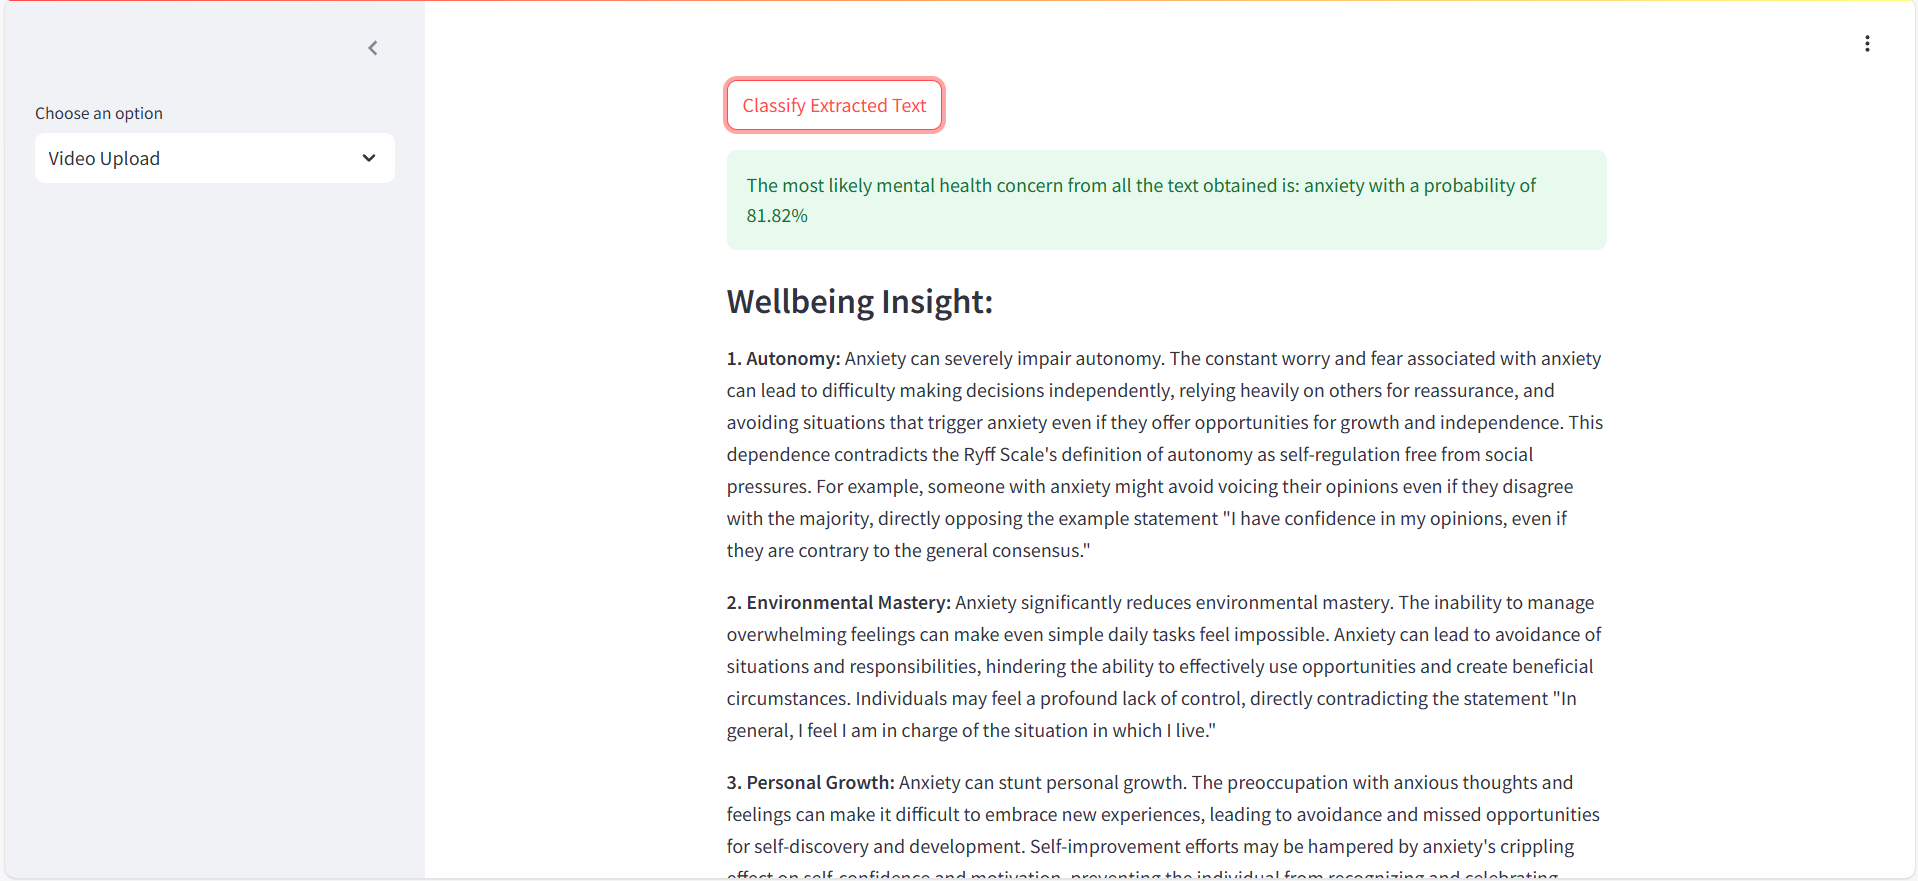
\includegraphics[width=0.8\textwidth]{App Images/13 Interface.png}  
    \caption{Video Classification Result}
    \label{06i}  % Label for referencing the figure
\end{figure}

\begin{figure}[h!]  
    \centering
    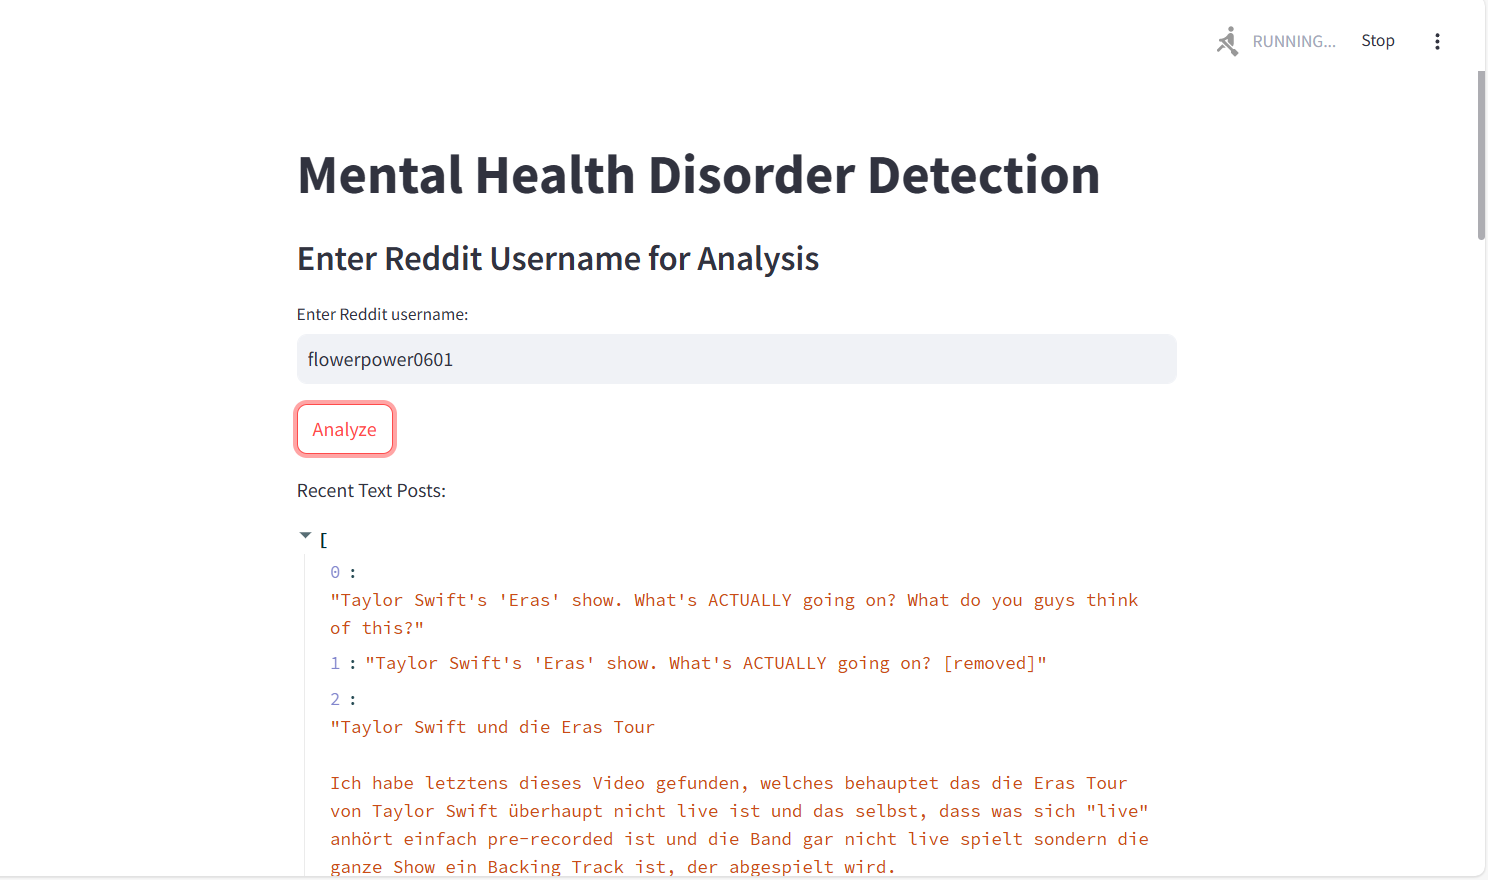
\includegraphics[width=0.8\textwidth]{App Images/06 Interface.png}  
    \caption{Reddit User Analysis}
    \label{07i}  % Label for referencing the figure
\end{figure}

\begin{figure}[h!]  
    \centering
    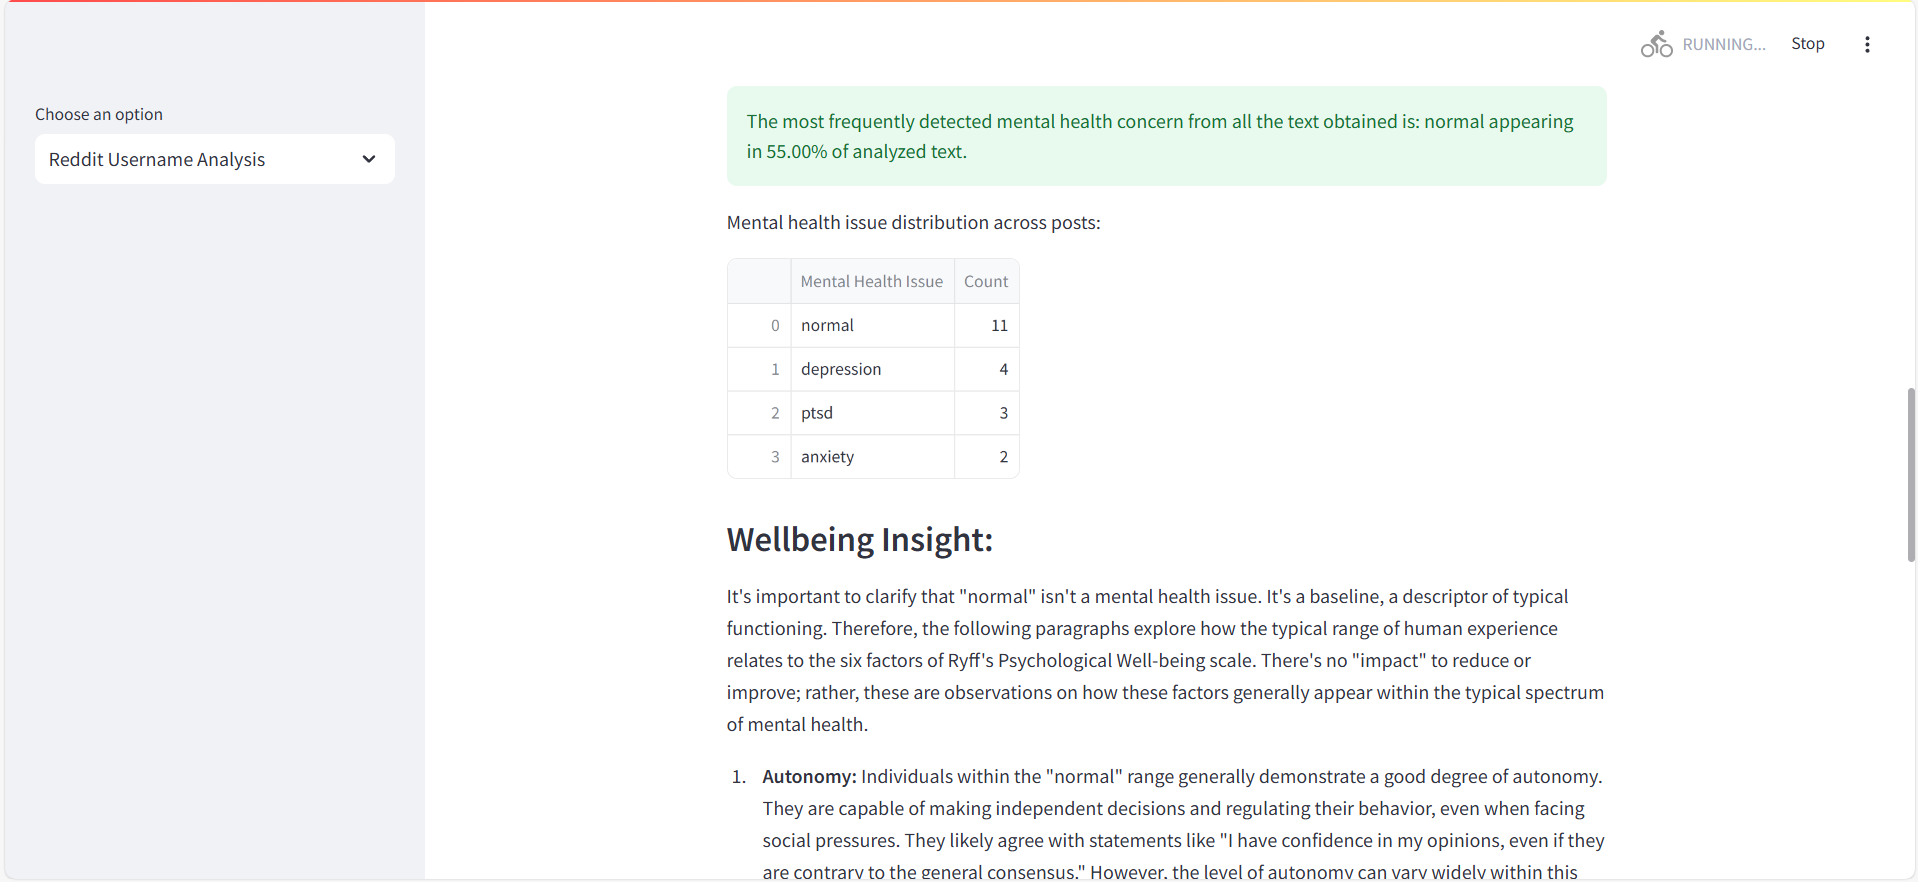
\includegraphics[width=0.8\textwidth]{App Images/07 Interface.png}  
    \caption{Result from Reddit Posts Analysis}
    \label{08i}  % Label for referencing the figure
\end{figure}


\begin{figure}[h!]  
    \centering
    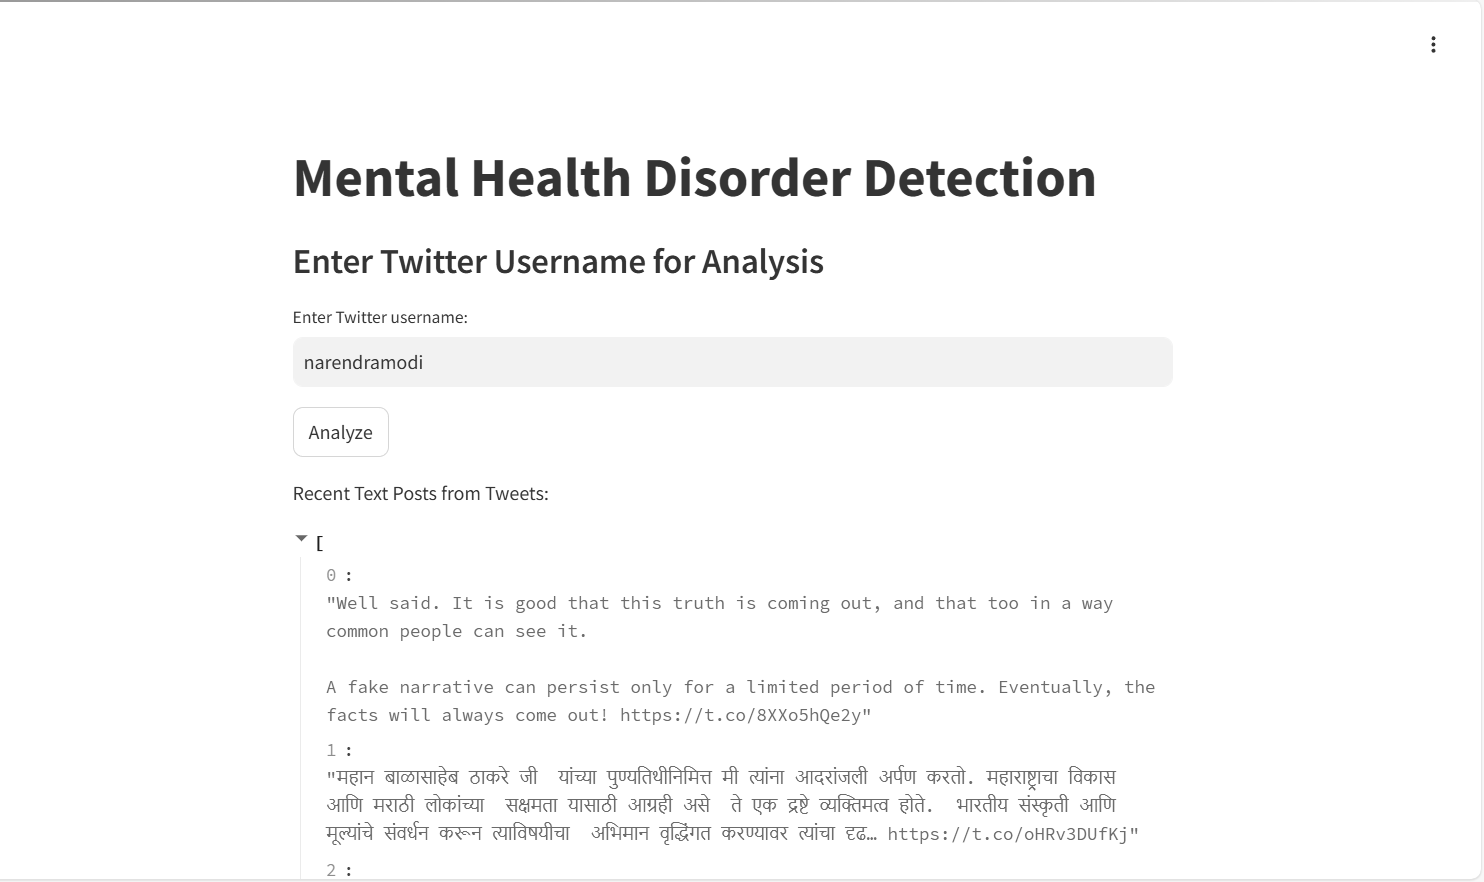
\includegraphics[width=0.8\textwidth]{App Images/08 Interface.png}  
    \caption{Twitter User Analysis}
    \label{09i}  % Label for referencing the figure
\end{figure}

\begin{figure}[h!]  
    \centering
    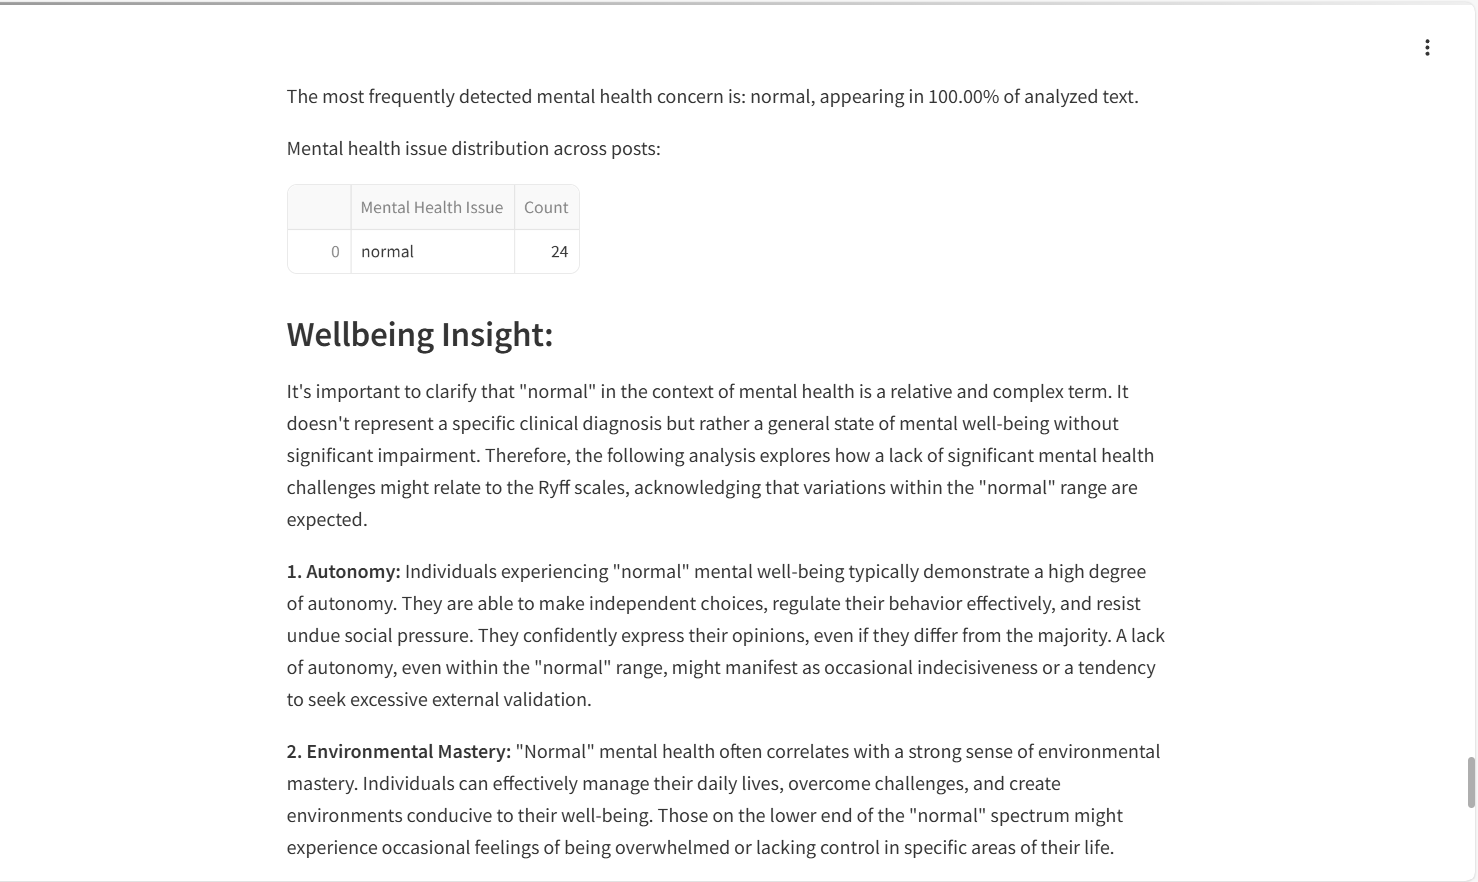
\includegraphics[width=0.8\textwidth]{App Images/10 Interface.png}  
    \caption{Result from Twitter Posts Analysis}
    \label{10i}  % Label for referencing the figure
\end{figure}

\begin{figure}[h!]  
    \centering
    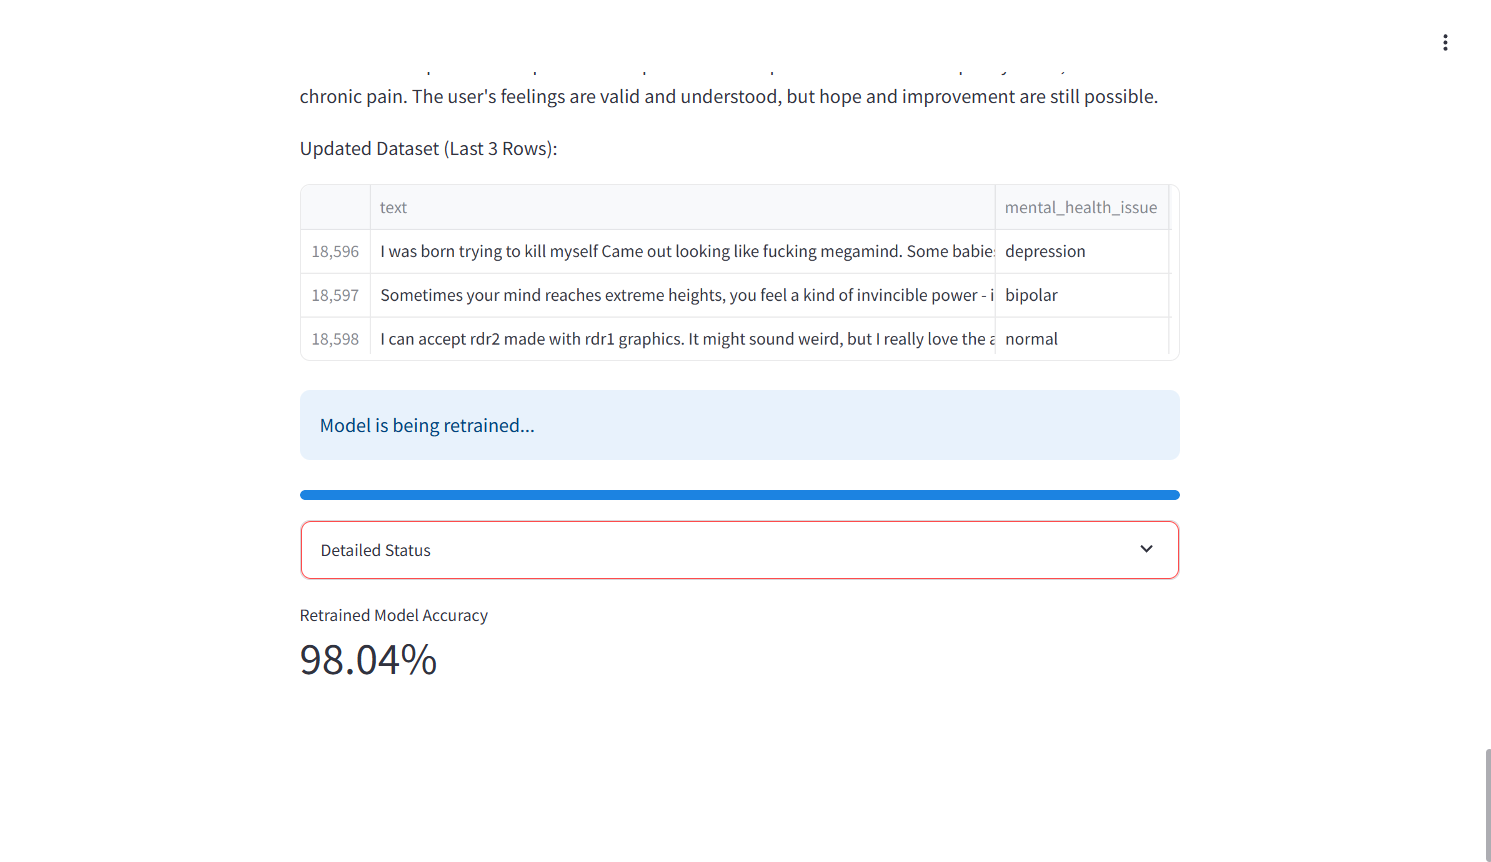
\includegraphics[width=0.8\textwidth]{App Images/17 Interface.png}  
    \caption{Result from Reddit Analysis and Model Retraining}
    \label{10i}  % Label for referencing the figure
\end{figure}

\begin{figure}[h!]  
    \centering
    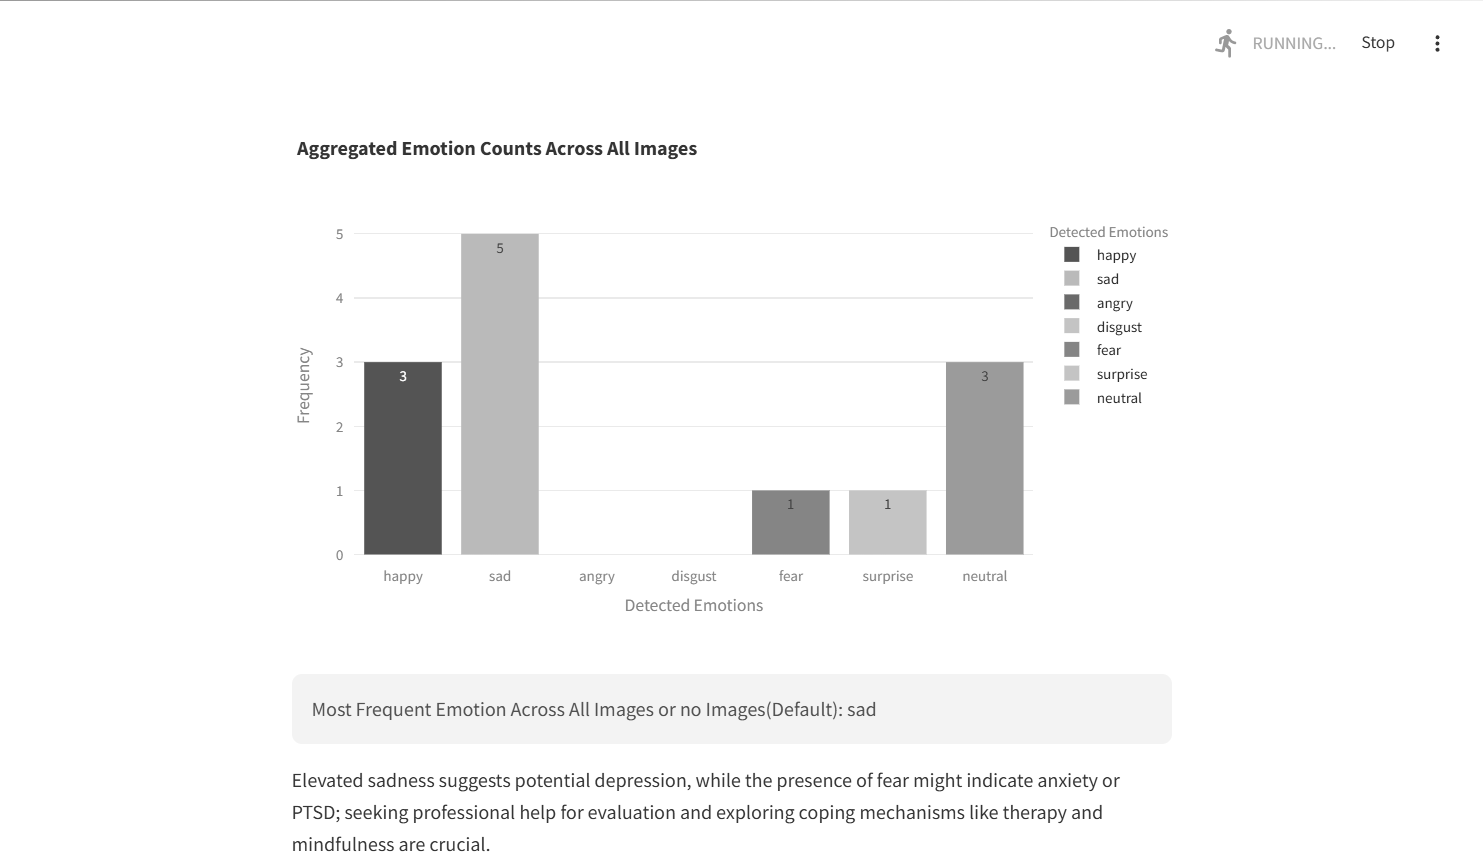
\includegraphics[width=0.8\textwidth]{App Images/12-1 Interface.png}  
    \caption{Result from the emotion analysis of facial expression}
    \label{10i23}  % Label for referencing the figure
\end{figure}

\begin{figure}[h!]  
    \centering
    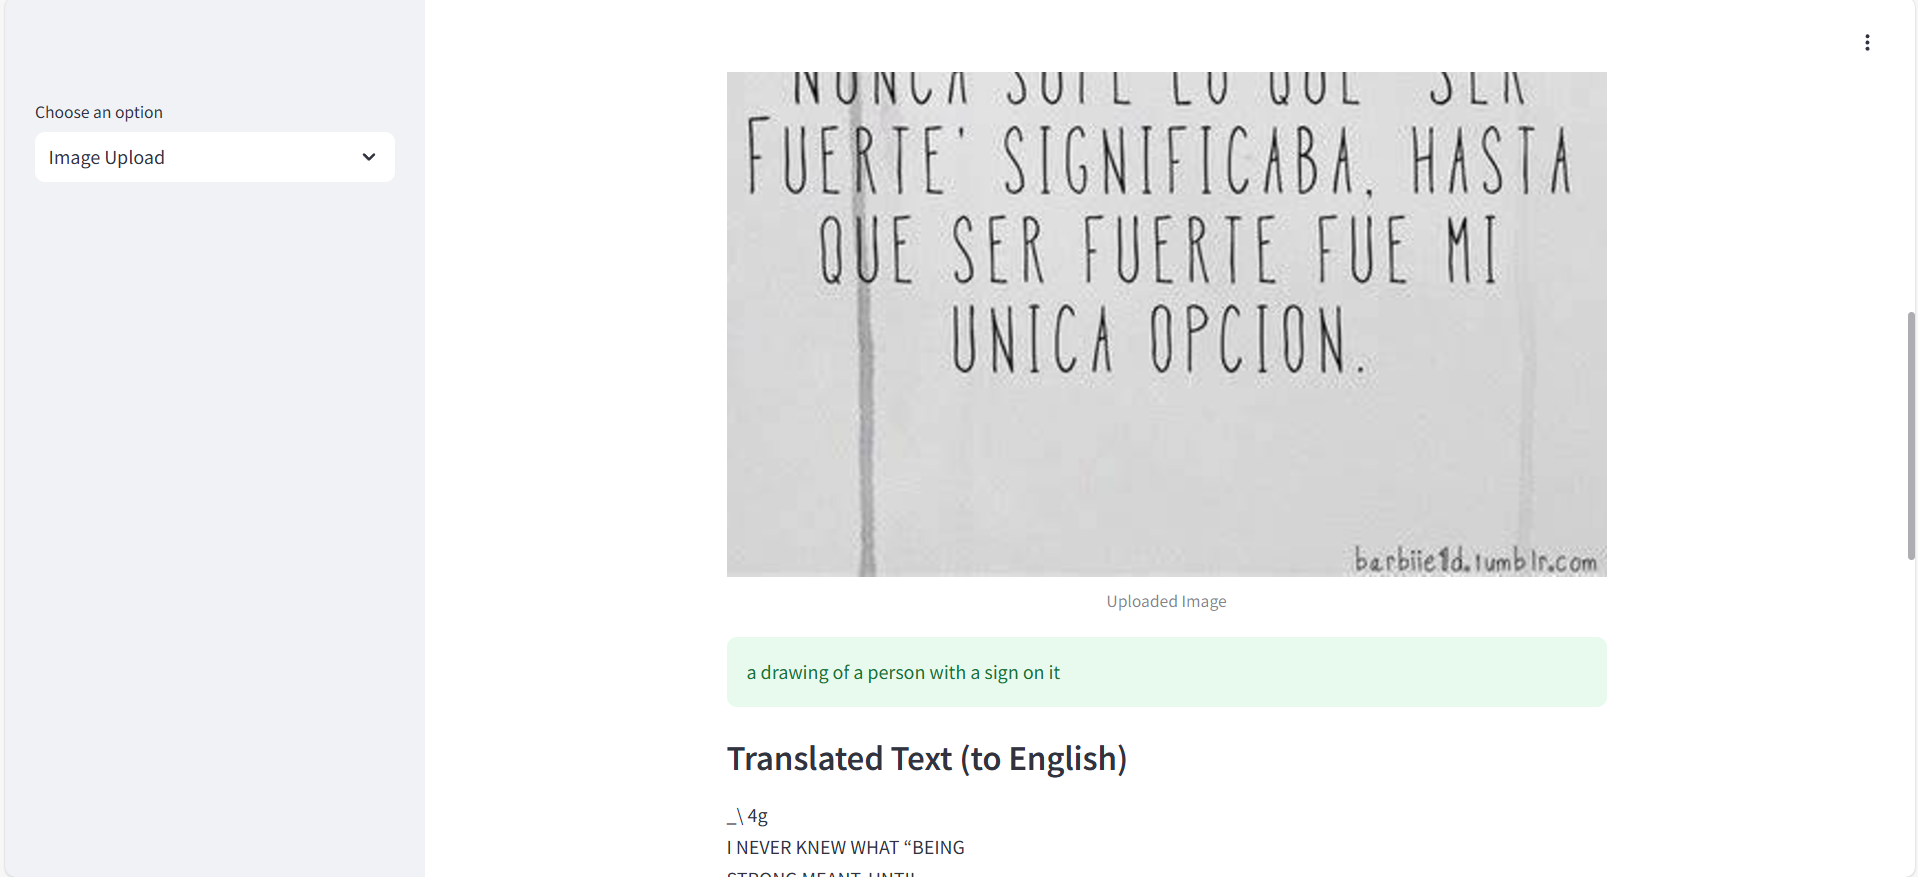
\includegraphics[width=0.8\textwidth]{App Images/18 Interface.png}  
    \caption{Generate Image Caption}
    \label{10i234}  % Label for referencing the figure
\end{figure}   

\begin{figure}[h!]  
    \centering
    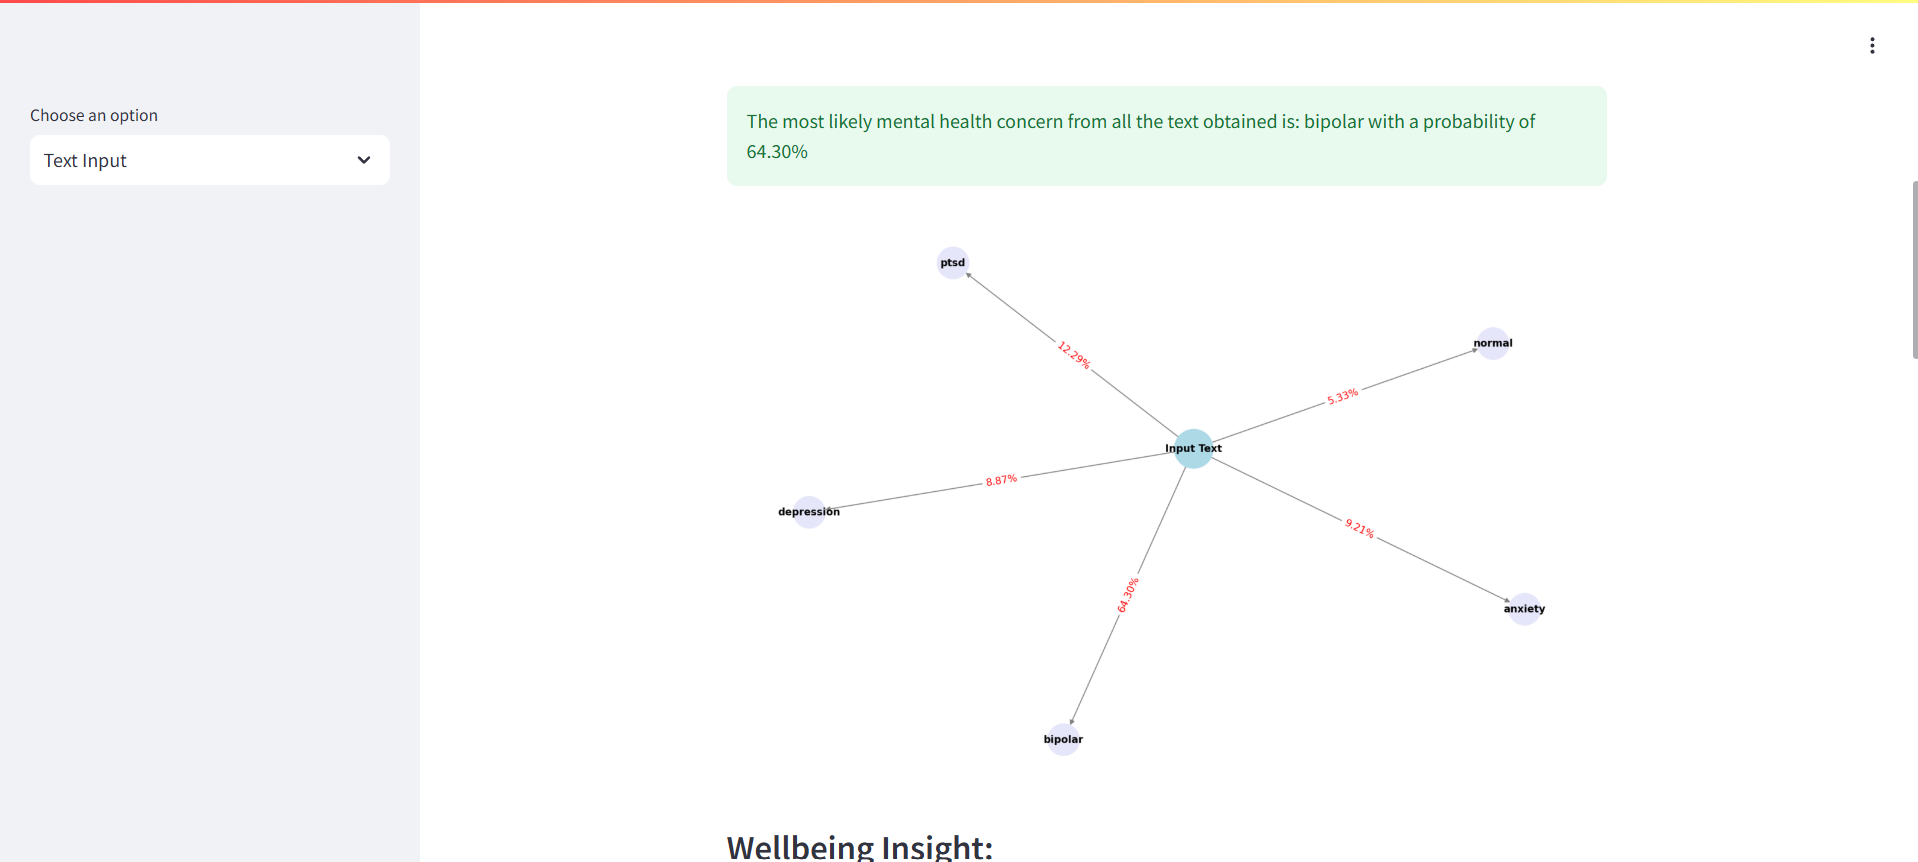
\includegraphics[width=0.8\textwidth]{App Images/19 Interface.png}  
    \caption{Knowledge Graph from classification}
    \label{10i23445}  % Label for referencing the figure
\end{figure}  







% ----------------------- Prototype ends -------------------


\begin{comment}

    \section*{APPENDIX B - Paper publications (optional) \label{sec:pubs}}
\addcontentsline{toc}{section}{APPENDIX B - Paper publications (optional)}
If any of your related paper(s) were published in a standard journal / presented in a recognized conference, mention the same including communication on your paper(s) acceptance / publishing note. You should also show appropriate documentation at the time of project viva.


\end{comment}

